\documentclass[border=3pt]{standalone}
% Shared preamble for every generated figure.
% Matches the report: newtx (Times), greyscale, square boxes.
\usepackage{newtxtext,newtxmath}
% newtx's typewriter (txtt) draws a slashed zero; use Latin Modern instead.
\renewcommand{\ttdefault}{lmtt}
\usepackage{tikz}
\usetikzlibrary{positioning,arrows.meta,calc,fit,backgrounds,shapes.geometric,
                decorations.pathreplacing,decorations.pathmorphing,matrix,patterns}

\definecolor{figgrey}{gray}{0.88}
\definecolor{figmid}{gray}{0.60}
\definecolor{figdark}{gray}{0.35}

\tikzset{
  fig/.style={font=\small},
  box/.style={draw,thick,minimum height=8mm,minimum width=22mm,align=center,
              inner sep=2pt,font=\small},
  greybox/.style={box,fill=figgrey},
  smallbox/.style={draw,minimum height=6mm,minimum width=16mm,align=center,
                   inner sep=2pt,font=\scriptsize},
  ln/.style={-{Stealth[length=2.2mm,width=1.8mm]},thick},
  lnb/.style={{Stealth[length=2.2mm,width=1.8mm]}-{Stealth[length=2.2mm,width=1.8mm]},thick},
  lbl/.style={font=\scriptsize,inner sep=1.5pt},
  note/.style={font=\scriptsize\itshape,inner sep=1.5pt},
}

\begin{document}
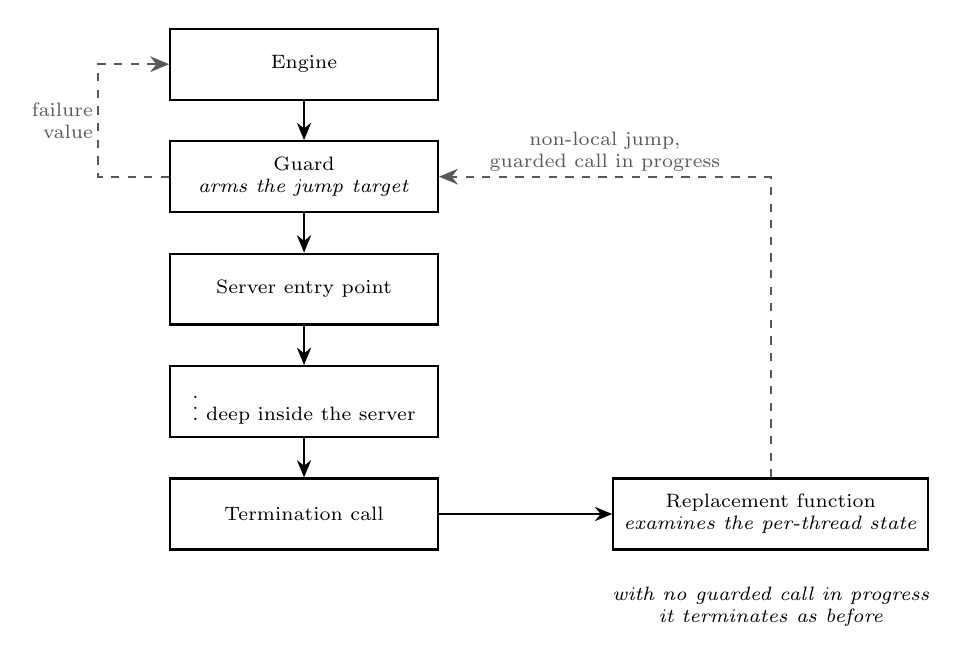
\begin{tikzpicture}[fig,
  fr/.style={draw,thick,minimum height=9mm,align=center,font=\scriptsize},
  ret/.style={-{Stealth[length=2.4mm,width=2mm]},thick,figdark,dashed}]

\node[fr,minimum width=34mm] (eng) {Engine};
\node[fr,minimum width=34mm,below=5mm of eng] (grd) {Guard\\\textit{arms the jump target}};
\node[fr,minimum width=34mm,below=5mm of grd] (ent) {Server entry point};
\node[fr,minimum width=34mm,below=5mm of ent] (deep) {\vdots\ deep inside the server};
\node[fr,minimum width=34mm,below=5mm of deep] (term) {Termination call};
\node[fr,minimum width=40mm,right=22mm of term] (repl) {Replacement function\\\textit{examines the per-thread state}};

\draw[ln] (eng) -- (grd);
\draw[ln] (grd) -- (ent);
\draw[ln] (ent) -- (deep);
\draw[ln] (deep) -- (term);
\draw[ln] (term) -- (repl);

\draw[ret] (repl.north) |- node[lbl,pos=0.75,above,align=center]{non-local jump,\\guarded call in progress} (grd.east);
\draw[ret] (grd.west) -- ++(-9mm,0) |- node[lbl,pos=0.25,left,align=right]{failure\\value} (eng.west);

\node[note,below=4mm of repl,align=center]
     {with no guarded call in progress\\it terminates as before};

\end{tikzpicture}
\end{document}
